\documentclass[12pt, a4paper, russian]{article}
\usepackage[margin=2cm]{geometry}
\usepackage[T2A]{fontenc}
\usepackage[utf8]{inputenc}
\usepackage[english,russian]{babel}
\usepackage{amsmath}
\usepackage{subfig}
\usepackage{caption}
\usepackage[compress]{cite}
\usepackage{graphicx}
\usepackage{xcolor}
\usepackage{algorithm}
\usepackage{algpseudocode}
\usepackage{enumitem}
\usepackage{multirow}
\usepackage{booktabs}
\usepackage{titling}
\usepackage[hidelinks]{hyperref}
\usepackage{setspace}
\singlespacing

% To prevent LaTeX from hyphenating
\tolerance=1
\emergencystretch=\maxdimen
\hyphenpenalty=10000
\hbadness=10000

\makeatletter \renewcommand*{\ALG@name}{Алгоритм} \makeatother


%%%%%%%%%%%%%%%%%%%%%%%%%%%%%%%%%%%%%%%%%%%%%%%%%%
\begin{document}

%%%%%%
%%%%%% Информация на английском языке
%%%%%%

\title{Global optimization algorithm using decision trees to find local extrema \thanks{The work was supported by the oneAPI Center of Excellence, by the Ministry of Science and Higher Education of the Russian Federation (project no. 0729-2020-0055), and by the Research and Education Mathematical Center (project no.  075-02-2021-1394).}}

\author{D.~I.~Silenko, I.~G.~Lebedev\\
	\small{Lobachevsky State University of Nizhny Novgorod, 603022, Nizhny Novgorod, Russia}
}
\date{}
\maketitle

\begin{small}
\textbf{Abstract:} The paper considers the solution of multidimensional global optimization problems using decision trees to identify areas of attraction of local minima. The local method is used for local refinement and is designed to speed up the convergence of the algorithm. The desired function satisfies the Lipschitz condition with an unknown constant. To confirm the theory, computational experiments were presented demonstrating acceleration when solving a series of test problems.

\textbf{Key words:} Global optimization, multiextremal functions, parallel computing, decision tree.
\end{small}

% References
\renewcommand{\refname}{References}
\bibliographystyle{IEEEtran}
\bibliography{articleEng}



%%%%%% 
%%%%%% Информация на русском языке
%%%%%%
\emptythanks
\title{Алгоритм глобальной оптимизации, использующий деревья решений для выявления локальных экстремумов\thanks{Работа выполнена при финансовой поддержке Министерства науки и высшего образования РФ (проект № 0729-2020-0055) и научно-образовательного математического центра “Математика технологий будущего” (соглашение № 075-02-2021-1394).}}

\author{Д. И. Силенко, И. Г. Лебедев\\
	\small{Нижегородский государственный университет им. Н. И. Лобачевского, 603022, Н.Новгород, Россия} 
}
\date{}
\maketitle

УДК 519.853.4

\vspace{\baselineskip}

\begin{small}
\textbf{Аннотация:} В работе рассматривается решение задач многомерной глобальной оптимизации с применением деревьев решений для выявления областей притяжения локальных минимумов. Локальный метод используется для локального уточнения и призван ускорить сходимость алгоритма. Для целевой функции задачи оптимизации предполагается только то, что она удовлетворяет условию Липшица, при этом константа считается неизвестной. Для подтверждения теории был приведен ряд экспериментов на серии тестовых задач,результаты демонстрируют значительное ускорение по числу итераций алгоритма.

\textbf{Ключевые слова:} деревья решений, глобальная оптимизация, многоэкстремальные функции, локальная оптимизация.
\end{small}


\section{Введение}

При нахождении глобального минимума функции можно использовать разные подходы: от алгоритмов использующих случайный поиск \cite{fio_bib1, fio_bib2, fio_bib3}, до детерминированного, гарантирующего нахождение глобального минимума \cite{. fio_bib4, fio_bib5, fio_bib6}. В реальных задачах, связанных с глобальной оптимизацией, любое вычисление значения функции является очень трудоемкой задачей, поэтому количество таких операций должно быть уменьшено. Это можно сделать путем целенаправленного выбора вариантов в процессе поиска наилучшего решения. На этой идее основан алгоритм глобального поиска (AGS). В статье мы попробуем объединить АГП и метод локальной оптимизации (метод Хука-Дживса) с помощью деревьев решений, с целью уменьшить количество проводимых итераций, а вместе с этим и количество вычислений целевой функции.

Алгоритмы локальной оптимизации предназначены для нахождения одного локального экстремума в области определения задачи, в котором целевая функция принимает  минимальное (или максимальное) значение. При их построении может использоваться как детерминированный спуск в области экстремальных значений, так и случайный поиск. К детерминированным относятся методы нулевого порядка и градиентные методы (первого и второго порядка).

Для того, чтобы понять, в какой момент лучше всего запускать локальный метод, мы используем алгоритм на основе деревьев решений. Мы накапливаем определенное число точек и лишь когда их станет достаточно начинаем обработку. Эти полученные точки мы используем для тренировки деревьев решений и предсказания по нему. Предсказание позволяет нам получить кусочно-линейную аппроксимацию по этому дереву. После чего мы рассматриваем уже полученную по дереву аппроксимацию. Проверяем значения соседних точек к той, которую считаем подозрительной на минимум, и оцениваем попали мы в область притяжения локального минимума или нет. 

\section{Постановка задачи}

Рассмотрим задачу глобальной оптимизации с целевой функцией $\varphi(y)$ на гиперинтервале $D=\{ y\in\ R^N:\ a_i\le\ y_i\le\ b_i,\ 1 \le\, i\le\ n \}$ Предположим, что функция удовлетворяет условию Липшица с заранее неизвестной константой $L$. Условие Липшица дает нам  ограниченные вариации значений функций при ограниченных изменениях её аргументов. При решение прикладных задач, это предположение можно интерпретировать как указание на ограниченную способность моделируемой системы к изменениям. 




\begin{equation} \label{sec:problem}   
\varphi(y^*) = min\{\varphi(y):y\in D\}, D = \{y \in R^N : a_i \leq y_i \leq b_i, 1 \leq i \leq N \},
\end{equation}
где $a,b \in R$ --- заданные векторы.


\begin{displaymath}
|\varphi(y_1)-\varphi(y_2)|\leq L\parallel y_1-y_2 \parallel
,y_1,y_2 \in D, 0<L< \infty.
\end{displaymath}




При численном решении задачи (\ref{sec:problem}) на основе некоторого числа $k$ вычислений значений целевой функции, происходит построение оценки $y_k^\ast\in D$,  соответствующей понятию близости к точке $y^\ast$ (например, ${ ||y^\ast -y}_k^\ast||\le\ \varepsilon$, где $\varepsilon\geq0$ — заданная точность). Для рассматриваемого класса задач предполагается, что оптимизируемая функция $\varphi(y)$ может быть задана алгоритмически как результат работы подпрограммы или библиотеки, а не аналитически в виде формулы.

По сравнению с другими типами задач оптимизации, задачи многоэкстремальной оптимизации имеют значительно более высокую сложность решения. Вычислительные затраты на решение задачи растут экспоненциально с увеличением размерности. Глобальная оптимальность является интегральным свойством решаемой задачи и требует исследования во всем пространстве поиска. В результате поиск глобального оптимума сводится к построению покрытия (сетки) в области параметров и выборе оптимального значения функции на этой сетке. 


\section{Многомерный алгоритм глобального поиска}

Алгоритм глобального поиска основан на идее, что минимизируемая функция представляет из себя случайный процесс. Решающее правило алгоритма построено так, что следующая итерация выполняется в глобальном минимуме математического ожидания значения функции. Найденная точка сохраняется в списке известных значений, после чего итерация повторяется . Это продолжается до тех пор, пока не будет достигнут один из выбранных критериев остановки: 
\begin{enumerate}
 \item Расстояние между двумя точками не будет меньше заданного значения.
 \item Новая точка не будут получена рядом с истинным глобальным минимумом.
 \item Будет достигнуто заданное максимального числа возможных итераций.
\end{enumerate}

При решении многомерных задач применяется редукция размерности (т.е. сведение многомерной задачи к эквивалентной одномерной) с использованием кривых Пеано. Которая позволяют свести исходную многомерную задачу оптимизации в области $D$  к одномерной задаче минимизации на отрезке $[0, 1]$

\begin{equation*}
\phi({y(x}^\ast))\ =\ min\{\phi(y(x)):\ x\epsilon[0,\ 1]\}
\end{equation*}
где функция  удовлетворяют уже равномерному условию Гельдера
\begin{equation*}
\left|\phi (y \left(x_1\right))- \phi (y \left(x_2\right)\right )|\le\ H\left|x_1-x_2\right|^\frac{1}{N},\ x_1,\ x_2\epsilon[0,1]		
\end{equation*}

Поэтому, не ограничивая общности, можно рассматривать минимизацию одномерной функции $f(x)\ =\ \phi(y(x)), \ x\epsilon [0,1]$, удовлетворяющей условию Гельдера.

Схема алгоритма:

На подготовительном шаге параллельно проводятся $p$ поисковых испытаний в произвольных внутренних точках $x^1, ...,x^p$ отрезка $[0,1]$, что соответствует первой итерации  алгоритма. 

Если выполнено $n\geq1$ итераций, которым соответствуют $k=k(n)$ проведенных поисковых испытаний в точках $x^i, 1\leq i\leq k$, то точки $x^{k+1},\ldots,x^{k+p}$ испытаний следующей $(n+1)$-й итерации будут определять следующим образом.

\begin{enumerate}

\item  Перенумеровать (нижним индексом) точки ранее проведенных испытаний $x^i, 1\leq i\leq k$, а также граничные точки отрезка [0,1] в порядке возрастания координаты:
 \begin{equation}
\label{agp1_sort}
	0=x_0<\ x_1<\ ...\ <x_{k+1}=1.
	\end{equation}
	и сопоставить им значения $z_i=f(x_i)$. 
	
\item  Вычислить текущие нижние оценки $M$ неизвестной константы Гельдера $H$:
 \begin{equation}
\label{agp2_mu}
	\mu=max\left\{\frac{|z_i-z_{i-1}|}{{{(x}_i-x_{i-1})}^{1/N}},\ i=1,\ldots,k\right\},\ M=\ \left\{\begin{matrix}r\mu,\ \mu>0,\\1,\ \mu=0,\\\end{matrix}\right.\
	\end{equation}
где $r>1$ --- параметр алгоритма.
   
\item  Для всех интервала $(x_{i-1},x_i), 1\leq i\leq k+1,$ вычислить значение $R(i)$, называемое \textit{характеристикой} интервала, в соответствии с формулами
\begin{equation}
\label{agp3_R1}
R(1)=2\Delta_1-4\dfrac{z_1}{M}, \; R(k+1)=2\Delta_{k+1}-4\dfrac{z_k}{M},
\end{equation}
\begin{equation}
\label{agp3_Ri}
R(i)=\Delta_i+\dfrac{(z_i-z_{i-1})^2}{M^2\Delta_i}-2\dfrac{z_i+z_{i-1}}{M},1<i<k+1,
\end{equation}
где \(\Delta_i=(x_i-x_{i-1})^\frac{1}{N}\).
   
\item   Упорядочить характеристики $R\left(i\right),\ 1\leq i \leq k+1,$ в порядке невозрастания 
\begin{equation}
\label{agp4_R_sort}
	R\left(t_1\right)\geq\ R\left(t_2\right)\geq...\geq\ R\left(t_k\right)\geq\ R(t_{k+1}),\ 
\end{equation}	
и выбрать интервал с номерами $t$, с наибольшими значениями характеристики.

\item  В выбранном интервале вычислить точку $x^{k+1}$, в соответствии с формулами
\begin{equation}
\label{agp5_x1}
	x^{k+j}=\frac{x_{t_j}+x_{t_j-1}}{2},\ t_j=1,\ t_j=k+1,
\end{equation}	
	\begin{equation}
\label{agp4_xi}	
	x^{k+1}=\frac{x_{t_j}+x_{t_j-1}}{2}-sign\left(z_{t_j}-z_{t_j-1}\right)\frac{1}{2r}\left[\frac{\left|z_{t_j}-z_{t_j-1}\right|}{\mu}\right]^N,\ 1<t_j<k+1.
\end{equation}	

\end{enumerate}

Отметим, что в прикладных оптимизационных задачах процесс проведения испытания является, как правило, значительно более трудоемким по сравнению с работой вычислительных правил алгоритма.

Алгоритм останавливает свою работу в случае, если значения $t$ из (\ref{agp4_R_sort}) выполняется условие \(\Delta_{t_j} < \varepsilon\). Данный критерий остановки (наряду с обычным для итерационных методов критерием, ограничивающим число выполненных итераций) используется в задачах оптимизации, в которых точка глобального минимума $x^*$ заранее неизвестна. 
	 
При решении тестовых задач, в которых точка глобального минимума $x^*$ является  известной, можно использовать также и критерий остановки по попаданию в окрестность глобального минимума. В этом случае алгоритм останавливает свою работу, если хотя бы для одного $t_j,\ 1\le\ j\le\ p$ из (\ref{agp4_R_sort}) выполняется условие $\left|x_{t_j}-\ x^\ast\right| < \varepsilon.$
	
Результатом работы АГП при решении рассматриваемой задачи, является оценка глобального оптимума:
\begin{equation}
f_k^*=\min_{1\leq i \leq k}f(x_i), \; x_k^*=arg \min_{1\leq i \leq k}f(x_i).
\end{equation}



В \cite{fio_bib20} приведено обоснование данного способа организации вычислений. А в работах  \cite{fio_bib9, fio_bib11} представлены модификации, учитывающие наличие ограничений-неравенств, а также информацию о значение производной целевой функции, 


\section{Метод Хука-Дживса}

 Метод Хука-Дживса представляет собой комбинацию поиска по образцу и исследующего поиска по направлениям  \cite{fio_bib14, fio_bib15}.


Алгоритм исследующего поиска состоит из следующих шагов: 
\begin{enumerate}
\item	Определяется значение шага (может меняться в процессе поиска и различно для каждой координаты).

\item	Шаг поиска будет успешным, если значения целевой функции в контрольных точках не превышают исходных значений целевой функции.

\item	В противном случае нужно вернуться к предыдущему пункту и сделать шаг в обратном направлении. 

\item	После того как будут пройдены все $N$ параметров, исследующий поиск заканчивается. Найденная точка называется базовой.
\end{enumerate}

Поиск по образцу состоит из выполнения одного шага от полученной базовой точки вдоль линии, соединяющей ее с предыдущей базовой точкой. Величина этого шага определяется задаваемым заранее параметром.



\begin{figure}[!h]
	\begin{center}
		\begin{minipage}[h]{0.8\linewidth}
			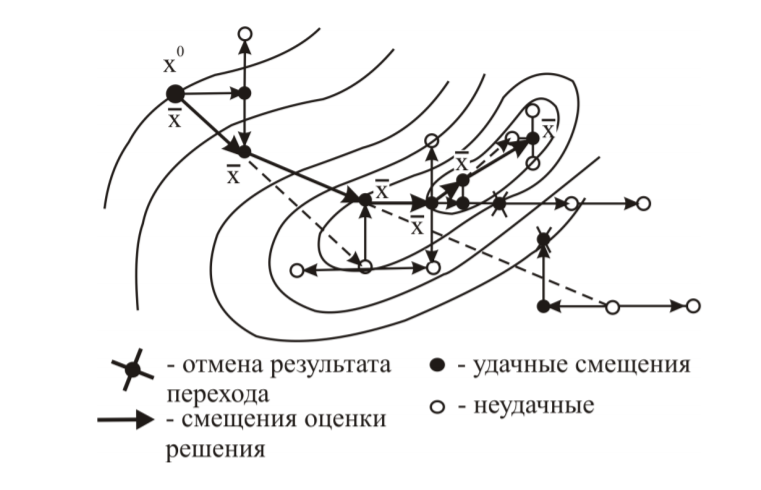
\includegraphics[width=1\linewidth]{figure/fig1.png}
			\caption{Пример итераций алгоритма Хука-Дживса} %% подпись к рисунку
			\label{fig:fig1}
		\end{minipage}
	\end{center}
\end{figure}	

\section{Деревья решений}

Деревья решений --- это метод автоматического анализа больших массивов данных, который применяется в машинном обучении. Деревья решений представляет собой бинарное дерево (дерево, в котором каждый не листовой узел имеет два дочерних узла). Его можно использовать как для решения задач классификации, так и для регрессионных задач. При решении задач классификации, каждый лист дерева помечается меткой класса, при этом несколько листьев могут иметь одну и ту же метку. В случае построение регрессии, каждому листу дерева присваивается константа, как следствие  получаемая функция аппроксимации является кусочно-постоянной.

Процедура прогнозирования по дереву решения начинается с корня. От каждого не листового узла процедура идет вправо или влево в соответствии со значением переменной (ее индекс хранится в наблюдаемом узле). 

Возможны следующие переменные:
\begin{enumerate}

\item Категориальные переменные --- значение дискретной переменной проверяется на предмет того, принадлежит ли оно определенному подмножеству значений (также хранящемуся в узле) из набора допустимых величин. Если принадлежит, то идем влево. В противном случае --- вправо. 

\item Упорядоченные переменные --- значения которых сравнивается с порогом (который также хранится в узле). Если значение больше порога, процедура идет вправо. В противном случае --- влево.
\end{enumerate}

Как только алгоритм достигает конечного узла, в качестве ответа процедуры прогнозирования выбирается значение, присвоенное этому узлу. 

В нашем случае дерево решений строит функцию $\varphi(y)$ кусочно постоянную аппроксимацию$\varphi(y)$  в многомерном пространстве, обозначим как $z' = \psi(y)$ значение вычисленное по decision tree в точке $y$.

При реализации алгоритма  решения задач многомерной глобальной оптимизации с применением деревьев решений для выявления областей притяжения локальных минимумов нами были использованы  деревья решений из библиотеки OpenCV (это библиотека алгоритмов компьютерного зрения, обработки изображений и численных алгоритмов общего назначения с открытым кодом). Подробнее с  деревьями решений можно ознакомиться в \cite{fio_bib16}


\section{Объединение локального метода и АГП в случае многомерных задач}

В текущем разделе приведем подробное описание того, как использовать деревьев решений в многомерном случае. В процессе работы АГП необходимо определить, стоит ли использовать текущую точку, в качестве стартовой для локального метода или нет. Для этого можно осмотреть соседние точки испытания и если среди них нет ни одной такой, значение функции в которой меньше, чем в текущей, то можно предположить, что мы находимся в области притяжения локального минимума и можно запустить локальный метод, чтобы быстрее сойтись к минимуму. Использование проекций многомерных точек на одномерный отрезок после редукции размерности (то, что позволяют сделать кривые Пеано) нам для этих целей не подойдут по нескольким причинам. Во-первых, функция после отображения сильно изменяется, один локальный минимум в многомерном пространстве может разделиться на множество минимумов после отображения. Во-вторых, после отображения мы можем потерять информацию о взаимном расположении точек исходной функции. Точки, расположенные близко в многомерном пространстве, могут оказаться на разных концах одномерного отрезка и наоборот).

%\begin{figure}[ht!]
%	\begin{center}
%		\begin{minipage}[h]{0.8\linewidth}
%			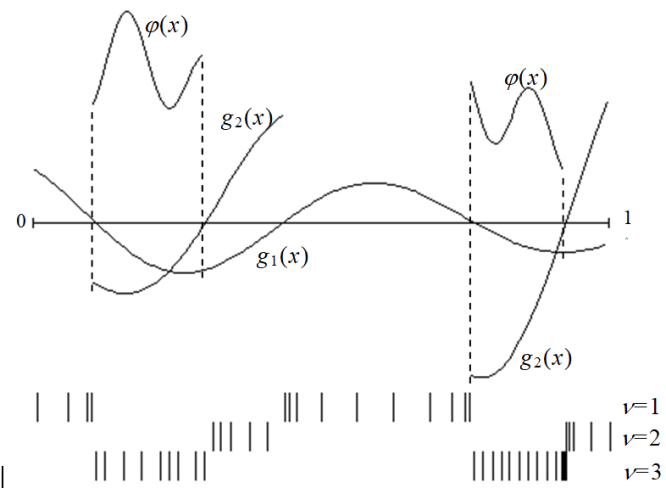
\includegraphics[width=1\linewidth]{figure/fig2.png}
%			\caption{Функция из генератора gkls до использования кривых Пеано} %% подпись к рисунку
%			\label{fig:fig2}
%		\end{minipage}
%	\end{center}
%\end{figure}	

%\begin{figure}[ht!]
%	\begin{center}
%		\begin{minipage}[h]{0.8\linewidth}
%			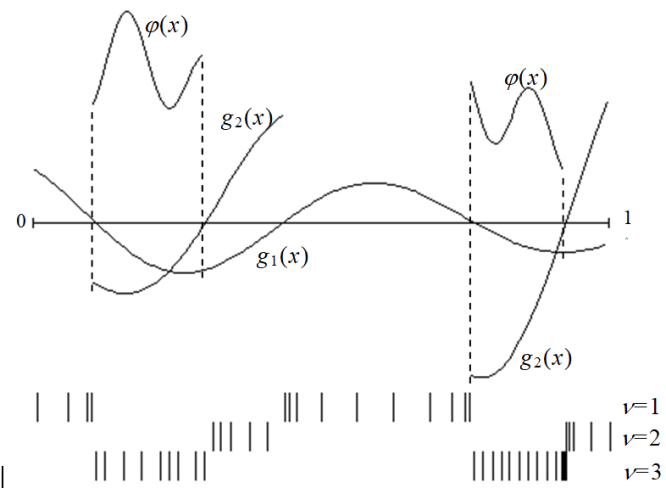
\includegraphics[width=1\linewidth]{figure/fig2.png}
%			\caption{Рисунок с двумерным деревом решений} %% подпись к рисунку
%			\label{fig:fig2_2}
%		\end{minipage}
%	\end{center}
%\end{figure}	


Поэтому мы будем работать именно с исходными точками. Однако определить соседние точки в многомерном пространстве достаточно трудоемко, и для этого мы будем использовать деревья решений. 

После проведения определенного числа испытаний (например, $100\ \ast\ N$), используем все накопившиеся точки для инициализации подходящей структуры данных и тренировки на ее основе дерева решений. Чтобы проще было определить соседние точки, мы построим равномерную сетку с определенным шагом по каждой из размерностей, после чего передадим эти точки на вход предсказанию по дереву. Теперь, имея равномерную сетку точек и зная значение функции в каждой из них, найдем ближайшую, с точки зрения евклидова расстояния, к исходной. Эта ближайшая точка является проекцией изначальной точки на равномерную сетку и что бы определить  ее соседей, достаточно  просто перебрать индексы соседей. К тому же поскольку дерево решений строит аппроксимацию исходной задачи (пусть и кусочно постоянную) мы можем оценить значение функции в тех областях, в которых испытания ранее не проводились.

При рассмотрении соседей необходимо учитывать следующее: если хоть один из соседей имеет значение функции меньшее, чем в текущей точке, то запуск локального метода не нужен; если какой-то из соседей имеет значение функции такое же, как в текущей, то его также необходимо проверить (найти всех его соседей и проверять их аналогично); и только в том случае, если все значения функций соседей больше (включая соседей равных точек) мы можем запускать локальный метод. Модифицированная версия алгоритма глобального поиска выглядит следующим образом:


\begin{enumerate}
	
\item  Перенумеровать (нижним индексом) точки ранее проведенных испытаний $x^i, 1\leq i\leq k$, а также граничные точки отрезка [0,1] в порядке возрастания координаты:
\begin{equation}
	\label{agp1_sort}
	0=x_0<\ x_1<\ ...\ <x_{k+1}=1.
\end{equation}
и сопоставить им значения $z_i=f(x_i)$. 

\item  Вычислить текущие нижние оценки $M$ неизвестной константы Гельдера $H$:
\begin{equation}
	\label{agp2_mu}
	\mu=max\left\{\frac{|z_i-z_{i-1}|}{{{(x}_i-x_{i-1})}^{1/N}},\ i=1,\ldots,k\right\},\ M=\ \left\{\begin{matrix}r\mu,\ \mu>0,\\1,\ \mu=0,\\\end{matrix}\right.\
\end{equation}
где $r>1$ --- параметр алгоритма.

\item  Для всех интервала $(x_{i-1},x_i), 1\leq i\leq k+1,$ вычислить значение $R(i)$, называемое \textit{характеристикой} интервала, в соответствии с формулами
\begin{equation}
	\label{agp3_R1}
	R(1)=2\Delta_1-4\dfrac{z_1}{M}, \; R(k+1)=2\Delta_{k+1}-4\dfrac{z_k}{M},
\end{equation}
\begin{equation}
	\label{agp3_Ri}
	R(i)=\Delta_i+\dfrac{(z_i-z_{i-1})^2}{M^2\Delta_i}-2\dfrac{z_i+z_{i-1}}{M},1<i<k+1,
\end{equation}
где \(\Delta_i=(x_i-x_{i-1})^\frac{1}{N}\).

\item   Упорядочить характеристики $R\left(i\right),\ 1\leq i \leq k+1,$ в порядке невозрастания 
\begin{equation}
	\label{agp4_R_sort}
	R\left(t_1\right)\geq\ R\left(t_2\right)\geq...\geq\ R\left(t_k\right)\geq\ R(t_{k+1}),\ 
\end{equation}	
и выбрать интервал с номерами $t$, с наибольшими значениями характеристики.

\item  В выбранном интервале вычислить точку $x^{k+1}$, в соответствии с формулами
\begin{equation}
	\label{agp5_x1}
	x^{k+j}=\frac{x_{t_j}+x_{t_j-1}}{2},\ t_j=1,\ t_j=k+1,
\end{equation}	
\begin{equation}
	\label{agp4_xi}	
	x^{k+1}=\frac{x_{t_j}+x_{t_j-1}}{2}-sign\left(z_{t_j}-z_{t_j-1}\right)\frac{1}{2r}\left[\frac{\left|z_{t_j}-z_{t_j-1}\right|}{\mu}\right]^N,\ 1<t_j<k+1.
\end{equation}	


\item  Получить вычисленное  значение функции с процесса $j$, добавить новый trial $z_j = f(y(x_j))$, к множеству $V$. 

%X_k=\left\{x^1,x^2,\ldots,x^{k+p}\right\}


\item 	Если $ k\ <\ 100\ast\ N$, то вернуться к шагу 1.

%\item 	Если используем decision tree не впервые, то перейти к пункту 15.

\item Создаем decision tree по множеству $I_k$, получаем функцию аппроксимации  $\psi(y)$.



\item 	Если используем decision tree впервые, то строим равномерную сетку

\begin{displaymath}
	Y'=\{ y'\in\ R^N:\ a_i\le\  {y'_i}^k \le\ b_i,\ 1\le\ i\le\ N,\ 1\le k\le\ \sqrt[N]{300}  \}
\end{displaymath}

\item 	Вычисляем значения аппроксимации: $Z' = \{ z'=  \psi(y'), y' \in Y'\}$

\item Для всех точек $y'\in V$:

Находим точку $y'_q$ ближайшую  к $y'$,

Производим обход соседей $y'_q$ по описанному ранее принципу.

Если ни у одной соседней точки не нашлось значений функции меньших, чем в $y'_q$, то запускаем локальный метод.

Очищаем множество $V$.


\end{enumerate}

%На рисунке  (\ref{fig:fig2}) отображены линии уровней оптимизационной задачи с отображением текущих  точек испытаний, и на рисунке  (\ref{fig:fig2_2}) отображено соответствующее дерево решений. 


Все полученные результаты были добавлены в систему globalizer \cite{fio_bib18}.
Если говорить более конкретно, то была реализована объединенная схема с запуском локальных методов в нужный момент, для чего была внедрена система  построения дерева решений, равномерной сетки и прочих сопутствующих вычислений.  
Ниже приведена блок-схема того, как данная схема была объединена с АГП.

\begin{figure}[ht!]

	\begin{center}
		\begin{minipage}[h]{0.9\linewidth}
			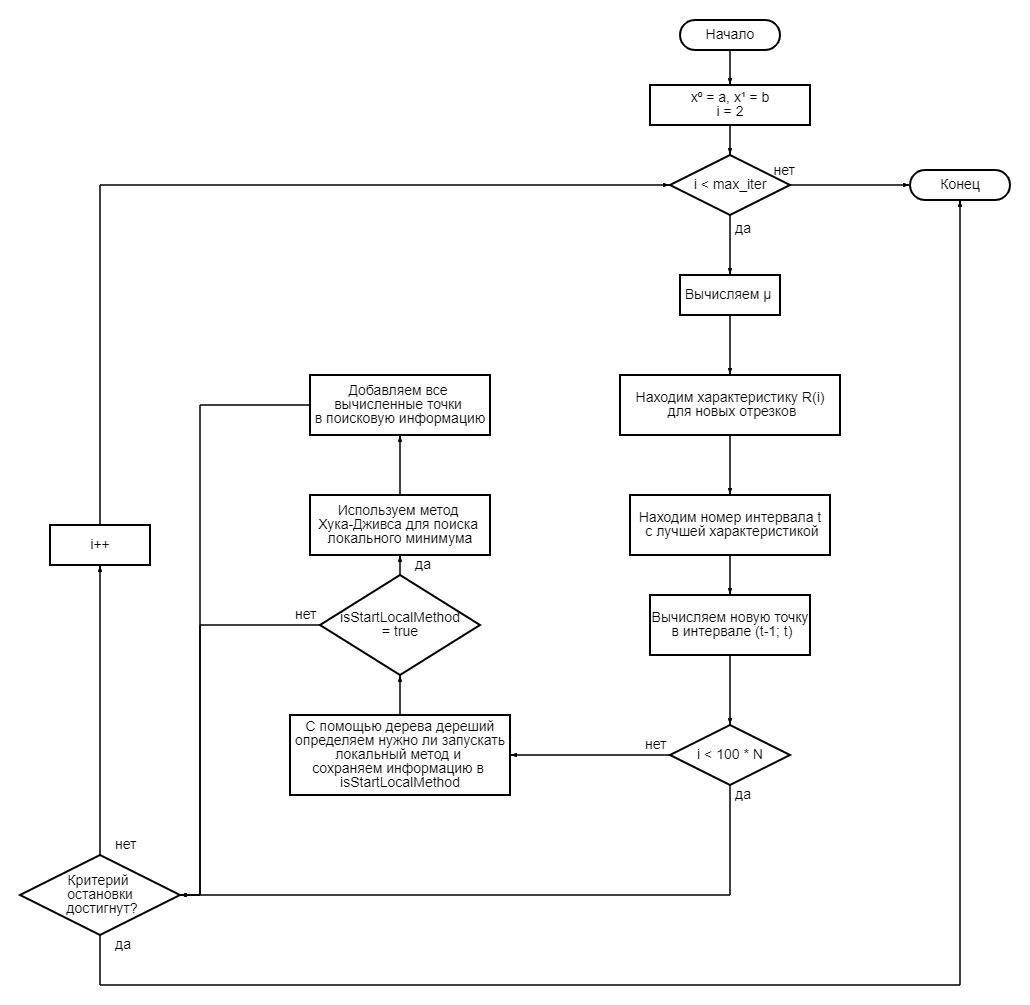
\includegraphics[width=1\linewidth]{figure/fig3.png}
			\caption{Блок-схема объединения АГП и метода Хука-Дживса с использованием дерева решений} %% подпись к рисунку
			\label{fig:fig3}
		\end{minipage}
	\end{center}
\end{figure}	

\section{Эксперименты}

Вычислительные эксперименты были проведены на компьютере со следующими характеристиками: операционная система Windows 11, процессор: Intel(R) Core™ i5-8250U CPU @ 1.60 GHz, 12 Gb RAM.

В работе \cite{fio_bib13, fio_bib17} описан GKLS-генератор, позволяющий порождать задачи многоэкстремальной оптимизации с заранее известными свойствами: количеством локальных минимумов, размерами их областей притяжения, точкой глобального минимума, значением функции в ней и т.п.


\cite{fio_bib13, fio_bib17} описывает генераторы GKLS, которые могут генерировать многоэкстремальные задачи оптимизации с известными свойствами: глобальным минимумом и его значением, количеством локальных минимумов и так далее.

В таблице \ref{tab:1} приведено среднее количество итераций методов глобальной оптимизации при решении серии задач из генератора GKLS. Знак «>» указывает на ситуацию, когда не все задачи были решены, в скобках указано количество нерешенных задач. Как видно, АГП превосходит методы DIRECT и DIRECTl по среднему числу итераций. 


\begin{table}[!ht]
    \caption{Среднее число итераций}
    \label{tab:1}
    \centering
    \begin{tabular}{|l|l|l|l|l|}
    \hline
        N & Problem class & DIRECT & DIRECTl & АГП  \\ \hline
        4 & Simple & >47282 (4) & 18983 & 11953  \\ \hline
        ~ & Hard & >95708 (7) & 68754 & 25263  \\ \hline
        5 & Simple & >16057 (1) & 16758 & 15920  \\ \hline
        ~ & Hard & >217215 (16) & >269064 (4) & >148342 (4)  \\ \hline
    \end{tabular}
\end{table}

В таблице \ref{tab:2} приведены результаты сравнения двух алгоритмов –-- многомерного алгоритма глобального поиска (АГП) и АГП с использованием деревьев решений для выявления областей притяжения локальных минимумов (Деревья решений). Численное сравнение проводилось на классах функций Simple и Hard размерности 2, 3, 4 и 5 из \cite{fio_bib19}. Алгоритм прекращал свою работу как только поражалась точка испытания в эпсилон окрестность истинного глобального минимума. 

\begin{table}[h!]
    \caption{Среднее число итераций и среднее число испытаний, проводимое разными алгоритмами}
    \label{tab:2}
    \centering
    \begin{tabular}{|c|c|c|c|c|c|}
    \hline
	
        N & Класс задачи & \multicolumn{2}{c|}{Среднее число итераций} & \multicolumn{2}{c|}{Среднее число точек испытаний} \\ \hline
          & ~ & АГП & Деревья решений & АГП & Деревья решений \\ \hline
          & Simple & 2350.0 & 247.4 & 2348.0 & 390.0  \\ \hline
        2  & Hard & 4732.3 & 353.6 & 4730.3 & 1101.1  \\ \hline
          & Simple & 2115.5 & 579.5 & 2113.5 & 2441.4  \\ \hline
        3  & Hard & 5347.4 & 588.1 & 5345.4 & 2532.7  \\ \hline
          & Simple & 12168.9 & 768.2 & 12166.9 & 3582.2  \\ \hline
        4  & Hard & 25636.5 & 960.0 & 52634.5 & 5171.6  \\ \hline
          & Simple & 20633.5 & 978.0 & 20631.5 & 4840.4  \\ \hline
        5  & Hard & 161094.9 (4) & 1217.0 & 161092.9 (4) & 7115.5  \\ \hline
    \end{tabular}
\end{table}

Ускорение по числу итераций достаточно велико, причем на задачах любой размерности. Среднее число точек испытаний тоже, практически везде, уменьшилось, но эти значения могут быть сильно выше, чем среднее число испытаний. Это связано с тем, что в точках испытаний учитываются и те точки, которые в процессе своей работы ставил локальный метод, а их может быть довольно много.


\section{Заключение}



В результате работы нами были успешно совмещены алгоритм глобального поиска с локальным поиском минимума (метод Гука-Джевса). Также были проведены вычислительные эксперименты на серии из сотни тестовых задач для экспериментального подтверждения теоретических свойств рассматриваемого алгоритма.

%
% ---- Bibliography ----
%
\renewcommand{\refname}{Список литературы}
\bibliographystyle{IEEEtran}   %%link to spmpsci.bst
\bibliography{article}        %%link to article.bib


\section*{Сведения об авторах}

\paragraph{Лебедев Илья Генадьевич} --- заведующий лабораторией, Нижегородский государственный университет им. Н.И. Лобачевского  e-mail: \url{ilya.lebedev@itmm.unn.ru}. Область профессиональных интересов: методы глобальной и локальной оптимизации, параллельные алгоритмы, программирование для графических процессоров, CUDA. Является автором и соавтором более 30 научных работ в указанных областях.

\paragraph{Д. И. Силенко} --- окончил бакалавриат института информационных технологий, математики и механики Нижегородского государственного университета им. Н. И. Лобачевского в 2021 году. В настоящее время является магистрантом института информационных технологий, математики и механики (направление - прикладная математика и информатика). Область научных интересов включает методы глобальной и локальной оптимизации, а также технологии параллельных вычислений и параллельные алгоритмы. e-mail: \url{dmsi@mail.ru}. Является автором или соавтором нескольких научных работ в указанных областях.



\paragraph{Контактный номер телефона:}{+7(910)898-02-39}

\section*{Authors' bio}

\paragraph{Ilya~G.~Lebedev} --- head of laboratory, Lobachevsky State University of Nizhny Novgorod. e-mail: \url{ilya.lebedev@itmm.unn.ru}. His research interests include algorithms of global and local optimization, parallel algorithms, GPU programming, CUDA. He has authored or coauthored more than 30 papers in these areas.

\paragraph{D. I. Silenko} --- Graduated the Institute of Information Technology, Mathematics and Mechanics of the Lobachevsky State University of Nizhni Novgorod in 2021. He is currently a master student of the Institute of Information Technology, Mathematics and Mechanics. His research interests are algorithms of global and local optimization, parallel algorithms and parallel technologies. e-mail: \url{dmsi@mail.ru}. He has authored or coauthored several papers in these areas.



\end{document} 